\documentclass[dvipdfmx]{jsarticle}
\usepackage[T1]{fontenc}
\usepackage[dvipdfmx]{hyperref}
\usepackage{lmodern}
\usepackage{latexsym}
\usepackage{amsfonts}
\usepackage{amssymb}
\usepackage{mathtools}
\usepackage{amsthm}
\usepackage{multirow}
\usepackage{graphicx}
\usepackage{wrapfig}
\usepackage{here}
\usepackage{float}
\usepackage{ascmac}
\usepackage{url}
\newtheorem{dfn}{定義}


\title{SATソルバーを用いた命題論理問題の説明と具体的問題に対する計算機実験}
\author{文理学部情報科学科\\5419045 高林 秀}
\date{\today}

\begin{document}

\maketitle

\begin{abstract}
本稿は、今年度論理と計算2における課題学習として「命題論理の説明」及び「SATソルバーを使用した、その具体的問題の解決を行う計算機実験」を行うものである。本稿の冒頭〜中盤では関係理論の説明を行い、終盤ではその理論を利用して、実際に具体的な問題をSATソルバーを使用して解答する。なお、本演習にはSATソルバーとしてclaspを使用した。
\end{abstract}

\section{目的}
本稿は、今年度論理と計算2における課題学習として、SAT ソルバーを用いた命題論理による宣言的問題解決を通じ,命題論理に関する学修内容を振り返ることを目的とする。\par
本稿は大まかに次のように構成される。
\begin{enumerate}
  \item 計算理論説明
  \begin{enumerate}
    \item 命題論理における解釈とモデル、その他関連する事項について
    \item SAT問題とはなにか
    \item DPLLアルゴリズムの解説
  \end{enumerate}
  \item 計算機実験
  \begin{enumerate}
    \item $N$人の女王
    \item グラフ頂点の彩色
  \end{enumerate}
  \item 各問に関する考察
  \item まとめ
  \item 巻末資料
\end{enumerate}
\section{計算理論説明}
この章では、今回の計算機実験に使用した各計算理論の解説を行う。
  \subsection{命題論理とは}
  まず命題論理とはなにか説明する。命題論理という言葉の意味はデジタル大辞泉に次のように書かれている。
  \begin{quote}
    記号論理学の基礎的部門。個々の命題を結合する「かつ」「または」「ならば」「でない」などの関係を、論理記号を用いて論理積(>)・論理和(<)・含意(→)・否定(~)などにより記号化して演算形式に表し、複合された命題を研究する学問。命題計算。
  \end{quote}
  そもそも命題は、数学では「真偽の判断の対象となる文章または式」であり、論理学においては「判断を言葉で示したもので真または偽」という性質を持つもの、という意味である。したがって、命題論理とは、命題同士の関係性を論理記号を使用して記号化し、演算できるようにしたものということだ。\par
  \paragraph{結合子}
  今説明したように、命題論理では命題同士の性質、関係性を扱う。それを説明する上で「結合子(論理記号)」と呼ばれるものが定義されている。
    \begin{table}[H]
      \centering
      \begin{tabular}{lll}
      記号                & 訳 & 意味\\
      $\wedge$          & 連言 & プログラミングではよくand、\&\&として扱われる。pかつq\\
      $\vee$            & 選言 & プログラミングではor, ||。pまたはq\\
      $\neg$            & 否定 & プログラミングではnot, !。pではない\\
      $\Rightarrow, \supset$     & 含意 &〜ならばの意味で使われる。直感的には「pが真であるとき、必ずqは真である」\\
      $\Leftrightarrow, \equiv$ & 同値 &「pはqである」がtrueのとき、もしくはその時点に限りtrueであるとき。pとqは同値。\\
      $\top$ &トートロジー(恒真)&後述するトートロジーを示す記号 \\
      $\bot$ &恒偽(矛盾)&後述する恒偽を示す記号\\
      (補足)$\veebar, \oplus$ & 排他的論理和& NANDと呼ばれるもの。\\
      \end{tabular}
  \end{table}
  \paragraph{命題文〜原子文,複合文}
  命題論理は次の要素から構成される。
  \begin{itemize}
    \item 文、命題文(sentence)※これは命題論理式とも言う。
    \begin{itemize}
      \item 原子文(atomic formula):これ以上分解することができない命題。最も単純な文。いわゆる1つの命題であり、以下の例のようにそれぞれ固有の記号で示すことができる。\par
      (例)$p$:「動物はいつか死ぬ」,$q$:「人間は動物である」,$z$:「人間はいつか死ぬ」
      \item 複合文(complex sentence):文同士を「結合子」で連結した文。命題同士の関係性を結合子を利用して連結し、新たな文を作ることができる。\par
      (例)$p \wedge q \Rightarrow z$:「動物はいつか死ぬ」かつ「人間は動物である」ならば「人間はいつか死ぬ」。
    \end{itemize}
  \end{itemize}
  まとめると、命題文には原子文や複合文と呼ばれる区分けが存在し、原子文は「真(true)、偽(false)、それ以上分解できない命題(記号)」であり、複合文は「命題文同士を結合子で連結した新たな命題文」ということになる。\par
  なお、true,falseと呼ばれる命題の真偽を示すこれらの記号は論理定数と呼ばれる。原子文の例で示した命題文を各記号に置き換えたもの$p,q,z$は命題記号ないしは命題変数と呼ばれる。\par
  \paragraph{命題文の構文}
  これらの要素を組み合わせて作られる命題文は、使用する結合子によって以下に区分けされる。
  \begin{itemize}
    \item 否定文:結合子$\neg$で連結されている複合文。
    \item 連言文:結合子$\wedge$で連結されている複合文。
    \item 選言文:結合子$\vee$で連結されている複合文。
    \item 含意文:結合子$\Rightarrow$で連結されている複合文。
    \item 同値文:結合子$\Leftrightarrow$で連結されている複合文。
  \end{itemize}
  とくに含意文$\alpha \Rightarrow \beta$については$\alpha$を前提、$\beta$を帰結と呼ぶ。また、原子文とその否定文$\neg p, \neg q, \neg z$をひとくくりにしてリテラルと呼ぶ。
  \paragraph{知識ベース}また、命題文の集合において、各文を結合子$\wedge$で連結したものを知識ベースと呼ぶことがある。(例:$KB$[KnowledgeBase] = \{S1, S2, S3\} $\Rightarrow$ S1 $\wedge$ S2 $\wedge$ S3)
  \paragraph{真理値表(trueth table)}
  命題文の真偽は先に上げた論理定数true, falseで示す。複合文の真偽を表にまとめて示したものを真理値表と呼ぶ。先に上げた各構文の真理値は、真理値表を用いて次のように定義されている。
\begin{dfn}
  複合文の真理値は以下のとおりである。
  \begin{table}[H]
      \centering
  \begin{tabular}{|l|l||l|l|l|l|l|} \hline
    $p$   & $q$   & $\neg p$ & $p \wedge q$ & $p \vee q$ & $p \Rightarrow q$ & $p \Leftrightarrow q$ \\ \hline
    false & false & true     & false        & false      & true              & true                \\ \hline
    false & true  & true     & false        & true       & true              & false               \\ \hline
    true  & false & false    & false        & true       & false             & false               \\ \hline
    true  & true  & false    & true         & true       & true              & true \\ \hline
  \end{tabular}
  \end{table}
\end{dfn}
上記真理値表より、含意文に関して重要なことを以下に列挙する。
\begin{itemize}
    \item 前提$\alpha$がfalseの場合、帰結$\beta$の真理値に関係なく、式としてtrueになる。
    \item 前提$\alpha$と帰結$\beta$の間に因果関係や関連性は要求されない。すなわち、前提文と帰結文がかけ離れた話題であっても、前提が真ならば含意文としては真となる。(例:$p:$のび太は人間である$\Rightarrow$ $q:$スネ夫は金持ちのボンボンである、の$p,q$に直接的な関連性はないが、前提の$p$がtrueであるので、文としてはtrue(正しい)となる。)
\end{itemize}
ここまで、基本用語の説明を行った。以降は、命題論理における「解釈、モデル、伴意関係」とはなにか、加えてSAT問題やDPLLアルゴリズムについて説明する。
\subsection{解釈について}
解釈という言葉の意味は日本国語大辞典に次のように書かれている(一部抜粋)。
\begin{quote}
  語句や物事の意味、内容などを説明すること。解き明かすこと。また、その解説。\par
  物事、特に表現されたものを、自分の経験や判断力などによって理解すること。\par
  法令の意味を明確にして、その内容が動かないように定めること。
\end{quote}
命題論理における「解釈」とは、これらの意味に関係なく次のように定義する。
\begin{dfn}
  命題文$\alpha$に現れる原子文(または命題記号)を$\alpha_{1},\alpha_{2},\alpha_{3},...,\alpha_{n}$とする。このとき、各原子文$\alpha_{i(1 \leq i \leq n)}$に対する真理値(truem false)の割当を「$\alpha$の解釈」と呼ぶ。
\end{dfn}
命題記号$p, q, r$が定義されているとする。このとき、命題文「$p \wedge q \vee r$」の解釈は次のものが考えられる。
\begin{align*}
  \{p=true, q=true, r=true\}, \{p=true, q=true, r=false\}, \\
  \{p=false, q=true, r=true\}, \{p=false, q=true, r=false\},\\
   \{p=true, q=false, r=true\}, \{p=true, q=false, r=false\},\\
    \{p=false, q=false, r=true\}, \{p=false, q=false, r=false\}
\end{align*}
そしてその組み合わせの数は$2^{3} = 8$より8個である。一般化すると、「$n$個の原子文がある時、解釈の個数は$2^{n}個$」である。\par
ただし、こうズラズラ書いていては非常に煩雑であるので、以下のようにtrueが割り当てられている命題記号だけ抜き出して記述する略記法も定義されている。上記例の場合は以下のようになる。
\begin{align*}
  \{p, q, r\}, \{p, q\}, \{q,r\}, \{q\},\{p,r\},\{p\},\{r\}
\end{align*}
すなわち、解釈とは命題記号に対するtrue,falseの割当パターンのことである。この解釈のうち、命題文$\alpha$の真理値をtrueにする解釈が、次に示す「モデル」と呼ばれる。
\subsection{モデルについて}
モデルという言葉の意味には次のようなものが挙げられるだろう。
\begin{itemize}
  \item ある事柄の手本や見本
  \item ある事象について、様々な要素とそれらの相互関係を定式化したもの
  \item 機械学習モデルなど、データ解析の手法のこと。
\end{itemize}
命題論理における「モデル」とは先に示したとおり、「命題文の真理値をtrueにする解釈」のことである。
\begin{dfn}
  命題文$\alpha$の真理値を真(true)にする解釈$I$を$\alpha$のモデルと呼ぶ。
\end{dfn}
繰り返すが、命題文をtrueにする解釈をモデルと呼ぶ、ただそれだけである。\par
真理値表では、各行がそれぞれ一つの解釈となっており、全体の命題文を真にする行(解釈)がモデルということだ。
\subsubsection{トートロジーと充足可能}
任意の命題文の真理値表を作成すると、すべての解釈でtrueになる命題文がでてくることがある。この様な命題文ないしは命題論理式を「トートロジー(tautology)」と呼ぶことがある。トートロジーとは日本語で「恒真」、すなわち常に真である、ということを意味する。以下、\url{https://qiita.com/kimunny/items/195f45154b6cc6a2940b}より引用する。
\begin{quote}
  命題論理において、パラメータの命題の値にかかわらず、常に真になる論理式をトートロジー、あるいは常真式と呼びます。
\end{quote}
以下にトートロジーになる命題論理式の例を示す。これらは後述する「命題論理式の標準形」に変形する際に必要となる考え方である。
%%ここにトートロジーの例を載せる
また、真理値表を書くとトートロジーであることが確認できる。
\begin{table}[H]
  \centering
\begin{tabular}{|c|c|c||c|c|c|c|c|c|c|} \hline
$\alpha$ & $\beta$ & $\gamma$ & $\alpha$ & $\vee$ & $(\beta \wedge \gamma)$ & $\Leftrightarrow$ & $(\alpha \vee \beta)$ & $\wedge$ & $(\alpha \vee \gamma)$ \\ \hline
false    & false   & false    & false    & false  & false                   & true              & false                 & false    & false                  \\ \hline
false    & false   & true     & false    & false  & false                   & true              & false                 & false    & true                   \\ \hline
false    & true    & false    & false    & false  & false                   & true              & true                  & false    & false                  \\ \hline
false    & true    & true     & false    & true   & true                    & true              & true                  & true     & true                   \\ \hline
true     & false   & false    & true     & true   & false                   & true              & true                  & true     & true                   \\ \hline
true     & false   & true     & true     & true   & false                   & true              & true                  & true     & true                   \\ \hline
true     & true    & false    & true     & true   & false                   & true              & true                  & true     & true                   \\ \hline
true     & true    & true     & true     & true   & true                    & true              & true                  & true     & true \\ \hline
\end{tabular}
\end{table}
\begin{table}[H]
  \centering
\begin{tabular}{|cc||cc|c|ccc|} \hline
$\alpha$ & $\beta$ & $\neg$ & $(\alpha \wedge \beta)$ & $\Leftrightarrow$ & $\neg \alpha$ & $\vee$ & $\neg \beta$ \\ \hline
false    & false   & true   & false                   & true              & true          & true   & true         \\ \hline
false    & true    & true   & false                   & true              & true          & true   & false        \\ \hline
true     & false   & true   & false                   & true              & false         & true   & true         \\ \hline
true     & true    & false  & true                    & true              & false         & false  & false \\ \hline
\end{tabular}
\end{table}
これとは反対に、どの解釈でも常に偽になる命題論理式を「矛盾(contradictory well-formed formula)」または「恒偽」と呼ぶ。\par
また、真にも偽にもなりうる命題論理式を「整合式(consistent well-formed formula)」または「充足可能」と呼ぶ。\par
これらの言葉を使うと、先に述べた論理定数であるtrueとfalseはそれぞれ、「トートロジー,恒偽」であり、任意の命題変数$p$はtrue,falseどちらも取り得るため充足可能である、と言える。
整理すると以下。
\begin{itemize}
  \item 論理定数true:トートロジーである。
  \item 論理定数false:恒偽である。
  \item 任意の命題変数$p$:充足可能である。
\end{itemize}
すなわち、ある命題文、命題論理式の真理値表を作成するということは「その命題文がトートロジーであるか、それとも恒偽であるか、それとも充足可能であるか」を調査、判定していることになる。
\subsection{伴意関係(Entailment)}
命題論理における伴意関係(別名:論理的帰結)とは以下のような意味をもつ。以下Wikipediaの\url{https://ja.wikipedia.org/wiki/%E8%AB%96%E7%90%86%E7%9A%84%E5%B8%B0%E7%B5%90}より引用する。
\begin{quote}
  論理的帰結(ろんりてききけつ、伴意、英: logical consequence, entailment)は、論理学における最も基本的な概念であり、複数の文(または命題)の集合と1つの文(命題)の間が「~だから、当然~」という繋がり方をする関係を指す。
\end{quote}
すなわち、「命題文の集合」と「命題文」の関係のことを示している。この伴意関係を式で示したものを「伴意式」と呼ぶ。このとき、命題文の集合のことを「理論」と呼ぶ。加えて、この「理論」は先に示した知識ベース「KB」のことであり、各命題文を連言記号で連結したもの「連言文」と同じである。
\paragraph{伴意式}一般的に伴意式は次のような表記をする。
\begin{align*}
  & G \models \alpha \\
  &意味:「理論Gを文(命題文)\alpha が伴意する」= 理論Gから\alpha が論理的に導出できる。\\
\end{align*}
これは、理論$G$の解釈がtrueであるとき、$\alpha$もtrueとなることを意味している。すなわち、$G$がtrueのとき、$\alpha$は常にtrueになるということだ。よって、含意文で示すと$G \Rightarrow \alpha がトートロジー$となる。つまり伴意関係とは、$G$がtrue($G$の全要素がtrue)であるとき、$\alpha$がfalseになることはありえない、トートロジーであると言っているのである。したがって、命題文が伴意関係にあるか否かはトートロジーであることを確認すればよいことになる。\par
例を挙げる。$G = \{p, q, (p \wedge q)\Rightarrow r\}としたとき、G \models r$または、$G$を展開して、$\{p, q, (p \wedge q)\Rightarrow r\} \models r$といったように表記する。このとき、$\{p, q, (p \wedge q)\Rightarrow r\}$は、$(p \wedge q \wedge (p\wedge q)\Rightarrow r)$と同じであるので、真理値表では以下のように示すことができる。
\begin{table}[H]
  \centering
\begin{tabular}{|ccc||c|c|c|} \hline
$p$   & $q$   & $r$   & $p \wedge q$ & $p\wedge q \Leftrightarrow r$ & $p \wedge q \wedge (p \wedge q \Rightarrow r)$ \\ \hline
false & false & false & false        & true                          & false                                          \\ \hline
false & false & true  & false        & true                          & false                                          \\ \hline
false & true  & false & false        & true                          & false                                          \\ \hline
false & true  & true  & false        & true                          & false                                          \\ \hline
true  & false & false & false        & true                          & false                                          \\ \hline
true  & false & true  & false        & true                          & false                                          \\ \hline
true  & true  & false & true         & false                         & false                                          \\ \hline
true  & ture  & true  & true         & true                          & true \\ \hline
\end{tabular}
\end{table}
以上より、$G$がtrueであるとき、$r$もtrueとなっていることが確認できる。したがって、伴意式「$G \models r$」は成立する(伴意関係にある)。
\subsection{SAT問題とは}
前章では、命題論理における解釈とモデルや伴意関係とはなにか、加えてトートロジーや恒偽、充足可能とはなにかについて説明してきた。この章では、先に示した「充足可能」についてより詳細に扱う。\par
初めに繰り返しになるが、「充足可能」とは「真にも偽にもなりうる命題論理式」のことであることは示した。ある命題論理式が充足可能であるか否かを判定するのが、SAT問題\footnote{・SAT:satisfiability problemの頭3文字\\・SAT問題:Boolean Satisfiability Testing}(充足可能性問題)である。より厳密には以下のように言われる※引用元\url{https://ja.wikipedia.org/wiki/%E5%85%85%E8%B6%B3%E5%8F%AF%E8%83%BD%E6%80%A7%E5%95%8F%E9%A1%8C}。
\begin{quote}
  充足可能性問題(じゅうそくかのうせいもんだい、satisfiability problem, SAT)は、一つの命題論理式が与えられたとき、それに含まれる変数の値を偽 (False) あるいは真 (True) にうまく定めることによって全体の値を'真'にできるか、という問題をいう。
\end{quote}
すなわち、与えられた命題論理式にモデルが存在するかを判定する問題ということになる。SAT問題は、命題論理式が以下のどちらに属するか決定する問題と言える。
\begin{itemize}
  \item モデルが存在する→充足可能
  \item モデルが存在しない→恒偽
\end{itemize}
これを利用して、背理法を使用して命題論理式にモデルが存在しないことを証明することもできる。\par
余談だが、このSAT問題は「NP完全\footnote{NP-complete problem:クラスNPに属する決定問題かつクラスNPに属する任意の問題から多項式時間還元可能な問題のこと。詳細な説明は本稿では扱わないが下記に参考URLを示す。
\begin{itemize}
  \item うさぎでもわかるP vs NP問題:\url{https://www.momoyama-usagi.com/entry/info-p-np}
\end{itemize}}」であることが最初に証明された問題でもあることが知られている。\par
では、実際どのように命題論理式にモデルが存在するか否かを求めるのかについて述べる。SAT問題は、与えられた命題論理式が充足可能かどうか言えれば良い。したがってまず思いつく手法としては先に示した「真理値表を作成する」という方法が思いつくだろう。しかし、真理値表はすべての命題変数に真理値を割り当てた後、解釈を見ることができる。したがって、論理式中の命題変数の個数が多ければ多いほど、充足可能かどうか判定するのに非常に時間がかかる。そこで、後述するSATソルバーと呼ばれるものが存在する。このSATソルバーは、単位伝搬やDPLLアルゴリズムなど様々な仕組みによって、効率よく命題論理式が充足可能かどうか判定することができる。単位伝搬やDPLLアルゴリズムについての説明は後述する。まずは、このSATソルバーを用いた問題解決システムである「SAT型システム」について紹介する。
\paragraph{SAT型システム}
与えられた問題をSAT符号化し、SATソルバーを使用して解くシステムをSAT型システムと言う。SAT型システムが生まれた背景としては、問題ごとに特化(適した)アルゴリズムを作成するのではなく、SAT符号化してSATソルバーに解いてもらおうとする考え方があった。問題ごとに特化(適した)アルゴリズムを作成するのは手間と時間がかかることがある。しかし、問題をSAT符号化すれば、SATソルバーに入力するだけで良いので、手間と時間がかからなくなる。他の問題に対しても、SATソルバーに対する入力を変更しさえすればよいので、前者よりもはるかに効率が良い。\par
近年、SATソルバーの解を求める性能が飛躍的に向上したこともあり、SAT型システムは以下のような分野において成功を収めている。
\begin{itemize}
  \item 自動テストパターン生成
  \item ソフトウェア検証
  \item 解集合プログラミング
  \item Linuxパッケージマネージャー(DNF)の依存性解決
\end{itemize}
この他にも多種多様な分野でSAT型システムは成功を収めている。他の事例については\url{https://www.jstage.jst.go.jp/article/jssst/35/4/35_72/_pdf}を参照いただきたい。
\subsubsection{SATの基本アルゴリズム}
\paragraph{木構造化}さて、先に示したとおり命題論理式がtrueになる解釈を調べる(モデルが存在するか否かを調べる)のがSAT問題である。問題を解くには各命題変数にtrue,falseの2通りの真理値を割り当てていくことになる。よって、命題変数をノード、真理値の割り当てを分岐として捉えることで「二分木」を作成することが可能になる。
\begin{figure}[H]
  \centering
  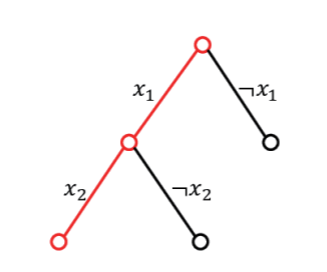
\includegraphics[scale=0.6]{cap1.png}
  \caption{SATの木構造化}
  ※引用元:\url{https://jssst-ppl.org/workshop/2017/slides/ppl2017_c4_soh.pdf}
\end{figure}
このように捉えることによって、木構造の特徴である「枝刈り」や「探索打ち切り」を行うことができる。SATソルバーはこのように、真理値割当中に命題論理式がtrueにならないと確定した時点で「探索打ち切り」や「分岐の削減」を行うことで効率を高めている。その方法が後述するDPLLアルゴリズムの章で触れる「早期停止」や「節学習」、「単位伝搬」と呼ばれる方法であり、それらを組み合わせたSATアルゴリズムが「DPLL」と呼ばれるアルゴリズムである。


SAT問題においては、モデルの有無のみが問われるので、探索中に1つのモデルが存在すればその時点で探索を終了すれば良いことになる。したがって、命題変数への真理値割当の際に命題論理式がtrueにならないことが確定した時点で探索を打ち切り、次の真理値割当へと進めば良い。

\subsection{DPLLアルゴリズム}
\section{計算機実験}
\subsection{実験準備}
  \subsubsection{実験環境}
  今回の実験は仮想マシン上でclaspのバイナリをダウンロードして行った。下記に実験時の環境を示す。
  \begin{itemize}
    \item ホストOS:Window10 Home 20H2
    \item 仮想OS:Ubuntu 20.04.2 LTS
    \item CPU:Intel(R)Core(TM)i7-9700K @ 3.6GHz
    \item GPU:Nvidia Geforce RTX2070 OC @ 8GB
    \item ホストRAM:16GB
    \item 仮想RAM:4GB
  \end{itemize}
\subsubsection{問題1:$N$人の女王}
配布資料中に、Processingのプログラムが「nQueen.pde」として以下の関数が用意されている。
\begin{itemize}
  \item バックトラック法を用いて nQueen を解く関数
  \item clasp への入力ファイルを作成する関数
\end{itemize}
\begin{enumerate}
  \item この問題に対するSAT符号化を詳細に説明せよ。
  \item N の大きさを様々に変えながら,バックトラック法で解いた場合と SAT ソルバーで解いた場合とでの実行時間を比較・考察しなさい.
\end{enumerate}
\subsubsection{問題2:グラフ頂点の彩色問題}
配布資料中の「GraphColoring」フォルダに、「都道府県の隣接関係」を表すグラフの頂点彩色問題の CNF ファイ
ルが用意されている。
\begin{enumerate}
  \item この問題に対するSAT符号化を詳細に説明せよ。
  \item 関東地方を対象に、いくつの塗分け方法があるか調べなさい。
  \item 47 都道府県を対象とした色塗りの例を一つ示しなさい。
  \begin{enumerate}
    \item (例)長野県:青色, 神奈川県:赤色、のように、どの都道府県をどの色で塗るのかを具体的に示すこと。
  \end{enumerate}
\end{enumerate}
\subsection{各問に対する解答・考察}
\subsubsection{問題1:$N$人の女王}
\subsubsection{問題2:グラフ頂点の彩色問題}
\section{まとめ}
\section{巻末資料}
本稿で使用した画像、プログラムコード等はすべて以下のリンク先に掲載している。必要に応じてご覧頂きたい。
\begin{itemize}
  \item GoogleDrive:\url{https://drive.google.com/drive/folders/1kOW_1KPUw_kBznaMWjge7HaBI7FoRAoq?usp=sharing}
  \item GitHub:\url{https://github.com/tsyu12345/logical_and_calculating_LectureCode/tree/master/No5}
\end{itemize}


\end{document}
